
\subsubsection{RNA processing}

Some polycistronic RNAs have to be cleaved before they become functional. This may be the case for some mRNAs, but is typical for sRNAs, tRNAs and rRNAs. The 30S RNA transcript of \textit{E. coli} undergoes several rounds of cleaving performed by different ribonucleases yielding a 9S, pre 16/17S and pre-23S intermediate before obtaining the 5S, 16S and 23S rRNA \citep{arraiano_critical_2010}. tRNAs also have to be cleaved at 3' 5' ends by a similar process involving several ribonucleases \citep{arraiano_critical_2010}. As for sRNA, their processing is globally unknown, except for a few examples.
\textcolor{red}{What level of detail do we want ?}

\subsubsection{RNA modifications}

\textcolor{red}{According to Karr, some bases of the RNAs are modified for proper folding and better coding recognition, but we have little data about it.}

\subsubsection{RNA decay}

There are two sides to RNA decay: the degradation machinery and possible determinants for targetting specific mRNA degradation. Let us start with the degradation machinery. There are numerous proteins that are able to cleave RNAs, some are more involved in RNA processing, some in degradation, but there is a large overlap in these activities \citep{arraiano_critical_2010}. We are only going to focus on the main ribonucleases generally considered as being responsible for global RNA degradation.

In \textit{E. coli}, the main enzyme is RNase E, an endonuclease that initiates degradation of RNAs. It seems to have two recognition pathways. Either the RNA has been modified on its 5'-end by the pyrophosphohydrolase RppH from 5' PPP to 5'P, enabling docking of the RNA by RNase E, or it may be recognized by associating with the C-terminal domain of RNase E, possibly using intermediates \citep{laalami_initiation_2013}. The latter case is not totally understood, numerous cofactors such as sRNAs, riboswitches or, more generally, ribosome depletion of the RNA could help recognition by RNase E. RNase E binds to the inner membrane, localizing RNA degradation at the cell periphery and is part of a structure called degradosome \citep{bechhofer_bacillus_2011,laalami_initiation_2013,bandyra_social_2013}. Its C-terminal domain is able to recruit another ribonuclease called PNPase that can slice RNAs in smaller parts through a 3'-5' exonuclease activity and other helper proteins such as the RNA helicase B (RhlB) and the glycolytic enzyme enolase. Once a RNA has been recognized by the degradosome and cleaved by RNase E, its degradation occurs very quickly. RhlB and PNPase or RNase II (with the help of the polyadenylation polymerase) can efficiently degrade secondary structures and an oligoribonuclease degrades remaining parts into single nucleotids (Fig. \ref{fig:rnaDegradation}). The process seems so efficient that degradation intermediates are not observed experimentally \citep{hambraeus_genome-wide_2003}.

In \textit{B. subtilis}, RNase E is not present. It has therefore been hypothesized that a similar ribonuclease is responsible for the initial cleaving of RNAs. RNase Y seems to fulfill this task \citep{lehnik-habrink_rna_2012,bechhofer_bacillus_2011,laalami_initiation_2013}. Due its recent discovery, some questions remain open. RNase Y seems to be able to bind to the membrane or to be part of a degradosome, but these asumptions have to be completely validated \citep{laalami_initiation_2013}. At the same time, another important ribonuclease was discovered, namely RNase J1, which is a 5'-3' exonuclease, which seems to be able to degrade RNAs alone, particularly 5' monophosphate RNAs (Fig. \ref{fig:rnaDegradation}) \citep{lehnik-habrink_rna_2012,bechhofer_bacillus_2011,laalami_initiation_2013}. RNase J1 probably also participates in degradation of fragments along with the PNPase as part of the degradosome. In other bacteria, any combination of RNase E, Y and J can be found but it seems that at least one of them is present \citep{archambault_measurements_2013}. The degradosome can also vary quite largely in composition \citep{laalami_initiation_2013}. For example, different specific ribonucleases or protein chaperones GroEL and DnaK can be recruited. It does also not necessarily bind to the membrane, e.g. in \textit{C. crescentus}, where DNA degradation seems to be located around the nucleoid, not at cell periphery.

\begin{figure}[!ht]
	\centering
	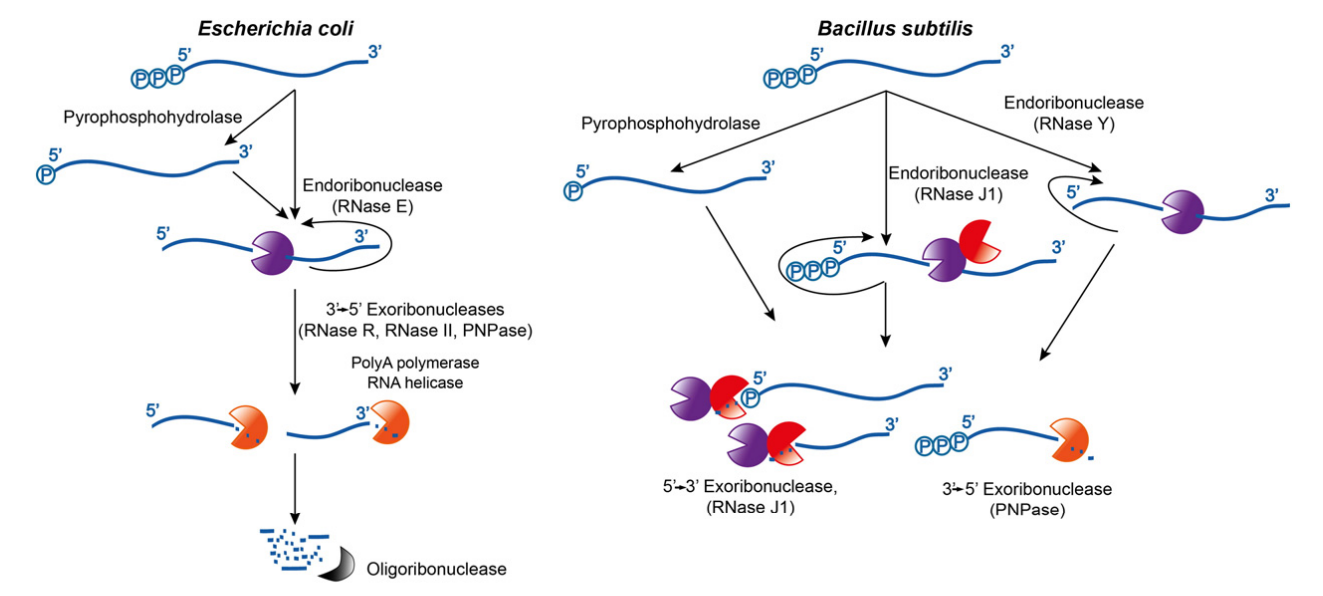
\includegraphics[width=0.9\linewidth]{figure/rnaDegradation}
	\caption{RNA degradation. Figure from \citet{bandyra_social_2013}.}
	\label{fig:rnaDegradation}
\end{figure}

RNA half-lives depend on the stability of the RNA, thus on its recognition by the degradosome or other ribonucleases. However, this stability is difficult to predict from the function of a gene, its sequence or even its secondary structure \citep{hambraeus_genome-wide_2003}. It is believed that ribosomes actively translating an mRNA protects it from being degraded by binding it, so that the RNA becomes unavailable for cleavage \citep{bandyra_licensing_2013}. Recent results shows that, while this is the case, it is not necessary to have ribosomes along the whole RNA, a ribosome can protect large parts of the mRNA "at distance" by making the docking of a specific part of the RNA impossible \citep{laalami_initiation_2013}. Whole genome studies yield distributions of RNA half-lives, showing that in \textit{B. subtilis}, most RNAs have a very short half-life (80\% shorter than 7 minutes) and a few have a relatively long half-life (3\% longer than 15 minutes) \citep{hambraeus_genome-wide_2003}. These half-lives probably vary depending on the physiological state of the cell. For example, targetting mRNAs with sRNAs is an efficient way to induce/inhibit translation (Fig. \ref{fig:srnaDegradation}).

\begin{figure}[!ht]
	\centering
	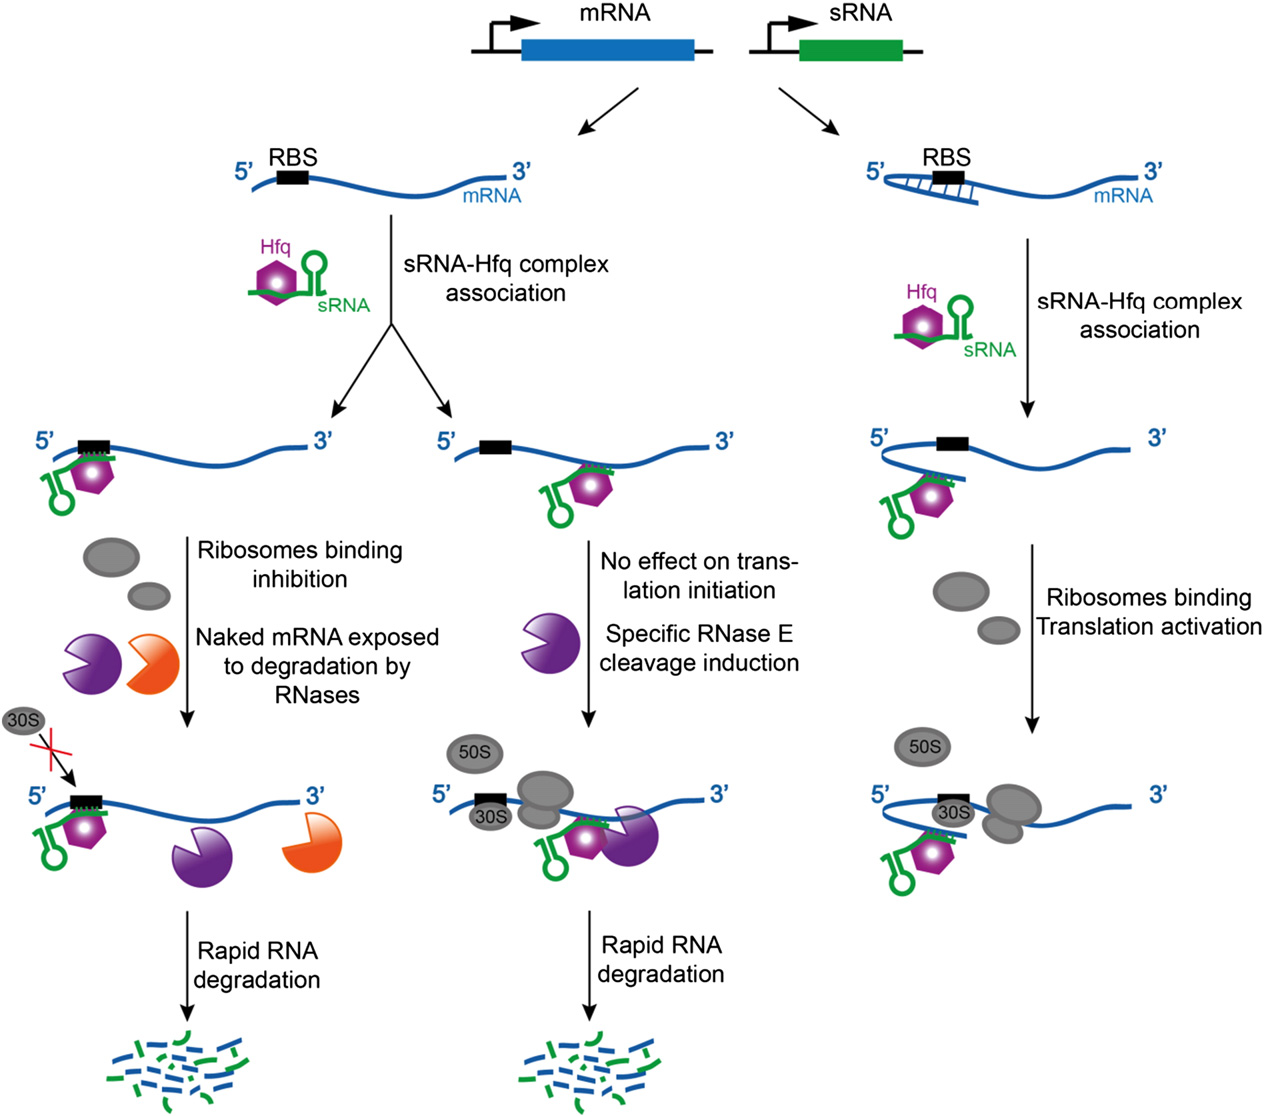
\includegraphics[width=0.9\linewidth]{figure/srnaDegradation}
	\caption{RNA control mediated by sRNAs. Figure from \citet{bandyra_social_2013}.}
	\label{fig:srnaDegradation}
\end{figure}